\documentclass{beamer}
\usepackage{beamerthemesplit} 
\usetheme{Warsaw}
\usepackage[spanish]{babel} 
\usepackage{ucs}
\usepackage[utf8]{inputenc}

\usepackage{amsthm}
\usepackage{amsmath}
\usepackage{amssymb}
\usepackage{esint}

\usepackage{siunitx}
\usepackage{physics}
\usepackage{graphicx}
\usepackage{xcolor}
\setbeamertemplate{navigation symbols}{}
\setbeamertemplate{footline}{% 
  \hfill% 
  \usebeamercolor[fg]{page number in head/foot}% 
  \usebeamerfont{page number in head/foot}% 
  \insertframenumber%
  %\,/\,\inserttotalframenumber
  \kern1em\vskip2pt% 
}
\definecolor{ao}{rgb}{0.0, 0.5, 0.0}
\begin{document}
\title{Un paseo por el espacio modular con lagrangianos especiales}  
\author{John Liu Anta\\
        Tutor: Wieland Staessens}
\date{6 de septiembre de 2017} 
\frame{\titlepage} 


\begin{frame}
  \frametitle{Objetivo}
  \begin{itemize}
    \item Teoría de cuerdas unifica las interacciones gauge con la gravedad
    \item Deseable obtener el Modelo Estándar a bajas energías
    \item Consideramos un formalismo concreto:
    Intersecciones de  D6-branas en la teoría Tipo IIA
    \textcolor{gray}{(Ibañez, Uranga '12)}
    \item Estudiamos las subvariedades sobre las que se enrollan las D6-branas (lagrangianos especiales):
      \begin{itemize}
        \item \textcolor{red}{Topología + Deformaciones}
        \item \textcolor{ao}{Intersecciones}
        \item \textcolor{orange}{Volumen}
      \end{itemize}
    \item En este trabajo, espacio compactificado en la quíntica aplicando la proyección orientifold
  \end{itemize}
\end{frame}

\begin{frame}
  \frametitle{Compactificaciones de la teoría Tipo IIA}
  \begin{itemize}
    \item Necesitamos reducir las 10 dimensiones a 4 dimensiones espacio-temporales
    \item Espacio total es $M_4\times X$, espacio interno una variedad de Calabi-Yau $X$
    \item Una \textbf{variedad de Calabi-Yau} (CY) es una variedad equipada con una estructura compleja $J$, una forma de Kähler $k$, una tres forma $\Omega_3$ y
      una métrica $g$ que satisface $R_{ab}[g]=0$
       Deformaciones de $k$ y $J$ definen el \textbf{espacio modular}.
       \textcolor{gray}{(Green, Schwarz, Witten '88)}
    \item Ejemplo CY: la \textbf{quíntica de Fermat}, una subvariedad de $\mathbb{CP}^4$
    \item $\mathbb{CP}^4$ se define como $(z_1,z_2,z_3,z_4,z_5)\in \mathbb{C}^5\backslash 0$ módulo la relación de equivalencia
      $(\lambda z_1,\lambda z_2,\lambda z_3,\lambda z_4,\lambda z_5)\sim (z_1,z_2,z_3,z_4,z_5)$
    \item La quíntica de Fermat se define como:
      \begin{equation*}
        z_1^5+z_2^5+z_3^5+z_4^5+z_5^5=0 
      \end{equation*}
  \end{itemize}
\end{frame}

\begin{frame}
  \frametitle{Compactificaciones de la teoría Tipo IIA}
  \begin{itemize}
    \item Otro punto del espacio modular de la quíntica es:
      \begin{equation*}
        z_1^5+z_2^5+z_3^5+z_4^5+z_5^5-5\psi z_1 z_2 z_3 z_4 z_5=0 
      \end{equation*}
      $\psi$ es complejo
    \item Compactificaciones de la teoría Tipo II en CY no permiten una teoría efectiva con fermiones quirales
    \item Necesario aplicar la \textbf{proyección orientifold}: tomamos el espacio cociente $X/\Omega \mathcal R$.
      $\Omega$ invierte la orientación de las cuerdas. $\mathcal R$ es una simetría $\mathbb Z_2$.\\
      En la quíntica $\mathcal R$ es la conjugación compleja de coordenadas: $z\to\bar z$
    \item Efecto de la proyección orientifold sobre el espacio modular:
      \begin{equation*}
        z_1^5+z_2^5+z_3^5+z_4^5+z_5^5-5\psi z_1 z_2 z_3 z_4 z_5=0 
      \end{equation*}
      $\psi$ ha de ser real
  \end{itemize}
\end{frame}


\begin{frame}
  \frametitle{D-branas}
  \begin{itemize}
     \begin{minipage}{0.8\linewidth}
    \item Elementos fundamentales de la teoría Tipo IIA: cuerdas abiertas y Dp-branas
    \item Dp-branas: generalización de cuerdas a objetos $(p+1)$-dimensionales
     \end{minipage}%
     \begin{minipage}{.2\linewidth}
        \centering
    %    \rule{.2\linewidth}{.2\linewidth}
      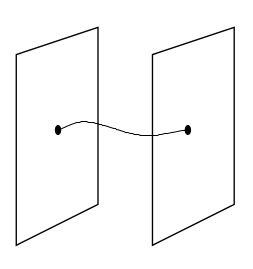
\includegraphics[width=\textwidth]{brane.png}
     \end{minipage}
    \item Consideramos solo D6-branas, se extienden en $M_4$ y se enrollan en 3 dimensiones internas
    \item Excitaciones de cuerdas abiertas con extremos en D6-branas describen partículas
    \item Cuerdas con extremos en $N$ D6-branas apiladas describen como partículas no masivas bosones gauge $U(N)$
    \item Cuerdas con extremos en una pila de $N_1$ D6-branas y otra de $N_2$ D6-branas que se intersecan
      se localizan en la intersección.
      Describen como partículas no masivas fermiones
      en la representación $(\mathbf{N_1,\bar N_2})$ de $U(N_1)\times U(N_2)$.
  \end{itemize}
\end{frame}

\begin{frame}
  \frametitle{Lagrangianos especiales en la quíntica}
  \begin{itemize}
    \item Las branas han de enrollarse en una subvariedad particular: \textbf{lagrangianos especiales} $\Pi$.
     Definidos como $k|_\Pi=0$ y $\Im(e^{-i\phi}\Omega)|_\Pi=0$.\\
     En la quíntica con la proyección orientifold, 125 lagrangianos especiales dados por puntos que satisfacen $z$ real.
     500 lagrangianos especiales adicionales se obtienen mediante rotaciones $\mathbb Z_5^4$: $z_i \to e^{i\frac{2\pi}{5}}z_i$\\
     \textcolor{gray}{(Becker, Becker, Strominger '95)}
   \item \textcolor{red}{La topología de los lagrangianos especiales obtenidos en la quíntica es $\mathbb {RP}^3$.
      Esta topología implica que los lagrangianos especiales no admiten deformaciones $\implies$ las branas se mantienen rígidas}
  \end{itemize}
\end{frame}

\begin{frame}
  \frametitle{Lagrangianos especiales en la quíntica}
  \begin{itemize}
    \item \textcolor{ao}{En la quíntica no hay ninguna intersección entre lagrangianos especiales que preserve la supersimetría $\implies$ No
      hay fermiones quirales.}\textcolor{gray}{ (Brunner et al. '00)}\\
      \textcolor{ao}{Solución posible: tomar combinaciones lineales de lagrangianos espaciales no supersimétricos} \textcolor{gray}{(Blumenhagen et al. '12)}
      \textcolor{orange}{
      \item Acoplo de la teoría gauge de la D-brana determinado por el volumen del lagrangiano especial: $V \sim 1/g^2$
    \item En la quíntica no sabemos resolver la integral del volumen.
      Limitamos el dominio de integración a las coordenadas positivas para obtener una cota inferior:
      %consideramos una cadena completa, y una combinación lineal podría dar lugar un ciclo
    }
    \begin{equation*}
  V \geq\frac{\Gamma\qty(\frac{1}{5})\Gamma\qty(\frac{3}{10})\Gamma\qty(\frac{11}{10})\Gamma\qty(\frac{6}{5})}{5 \times 2^{1/5}\pi}\approx 0.61
    \end{equation*}
  \end{itemize}
\end{frame}

\begin{frame}
  \frametitle{Deformaciones de la quíntica}
  \begin{itemize}
    \item Hay 101 deformaciones posibles de la quíntica de Fermat. 
      Consideramos
      \begin{equation*}
        z_1^5+z_2^5+z_3^5+z_4^5+z_5^5-5\psi z_1z_2z_3z_4z_5=0 
      \end{equation*}
      \textcolor{red}{
    \item Propiedades topológicas permanecen invariantes: rigidez de los lagrangianos especiales, no hay intersecciones}
    \textcolor{ao}{
    \item El volumen depende de $\psi$. Comparamos la cota inferior del volumen dividiendo entre el volumen sin deformar}
      \begin{equation*}
        V_\psi/V \approx 1 - 0.21\psi -0.01\psi^2+O(\psi^3)
      \end{equation*}
      \begin{center}
      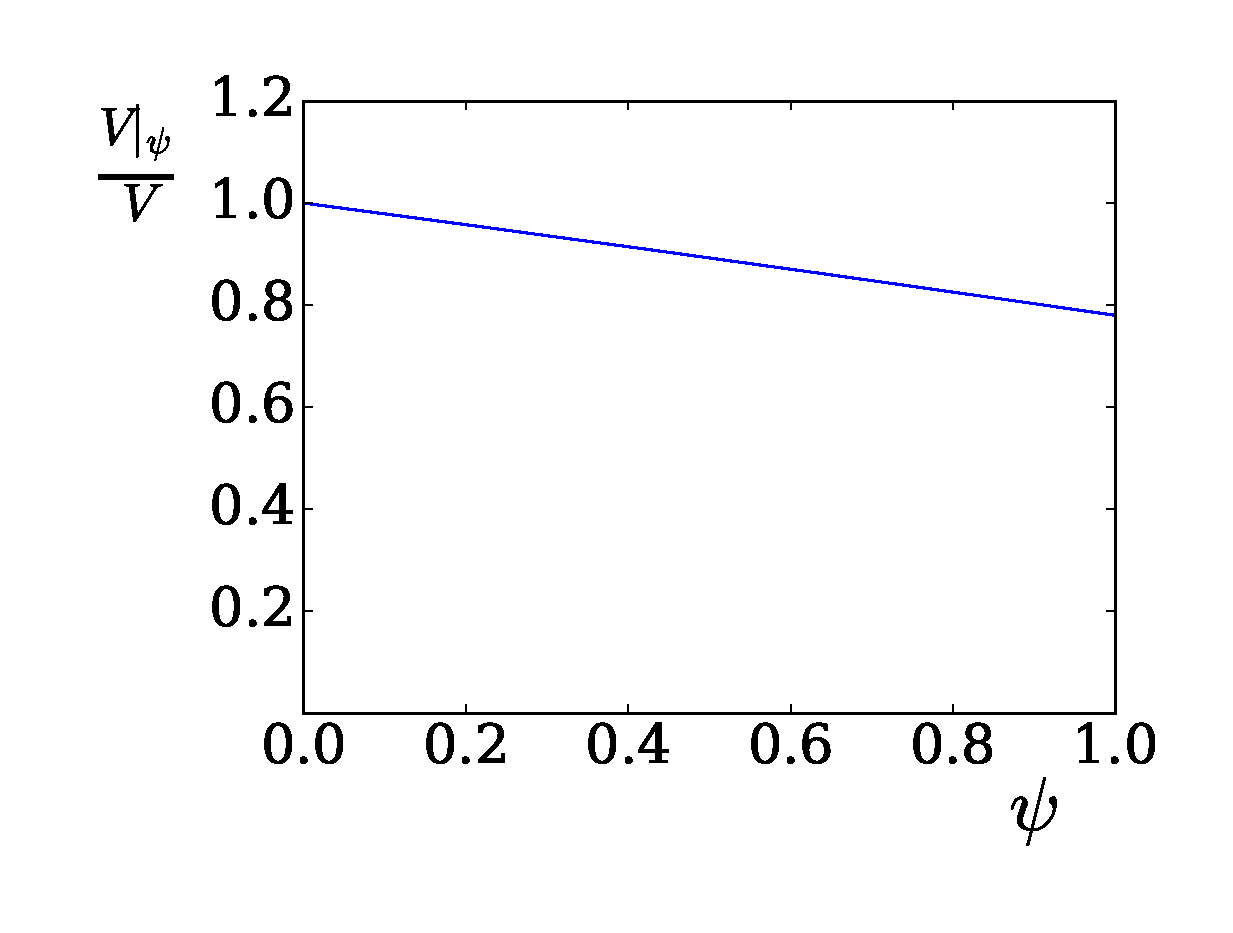
\includegraphics[width=0.4\textwidth]{graph.eps}
      \end{center}
  \end{itemize}
\end{frame}

\begin{frame}
  \frametitle{Conclusión}
  \begin{itemize}
    \item Lagrangianos especiales supersimétricos en la quíntica son rígidos.
      Sin embargo, nunca se intersecan, por lo que no describen fermiones quirales
    \item  Podríamos aplicar un tratamiento similar para otras compactificaciones
    \item Interesante estudiar el resto de deformaciones de la quíntica y un método para el cálculo preciso 
      del volumen de los lagrangianos especiales
  \end{itemize}
\end{frame}

\begin{frame}
  \begin{center}
  \Large{GRACIAS POR VUESTRA ATENCIÓN}
  \end{center}
\end{frame}

\begin{frame}
  \frametitle{Deformaciones de lagrangianos especiales}
  \begin{itemize}
    \item 
  \end{itemize}
\end{frame}

\end{document}

